% Лабораторная работа по криптографии № 3
% Дуников Константин Артёмович 

% Тип документа: статья, на бумаге А4
\documentclass[a4paper]{article}

% Подключение сторонних tex файлов 
\usepackage{import}


% Основные данные - ВУЗ, факультет, город...
\import{./../../stuff/tex}{config.tex}
% Небольшой набор инструментов
\import{./../../stuff/tex}{tools.tex}

% Подключение необходимых зависимостей
\import{./../../stuff/tex/settings}{packages.tex}
% Настройка подключенных пакетов
\import{./../../stuff/tex/settings}{preferences.tex}


% Шаблон титульной страницы 
\import{./../../stuff/tex/templates}{title.tex}
% Упрощенный блок "выполнил"
\import{./../../stuff/tex/templates}{sign2.tex}
% Макрос для содержания
\import{./../../stuff/tex/templates}{toc.tex}

% Определяем название документа
\title{
  ОТЧЕТ \\
  О ПРАКТИЧЕСКОЙ РАБОТЕ №1 \\
  по дисциплине <<Криптографические методы защиты информации>> \\
  Криптосистемы с открытым ключом
}
% Указываем преподавателя
\renewcommand{\teachername}{
    Заведующий кафедрой информационной безопасности киберфизических систем \\
    канд. техн. наук, доцент \\
    О.О. Евсютин
}

\setminted{fontsize=\footnotesize,baselinestretch=1}

% Путь до внешних изображений
\graphicspath{ {./figures/}}
% Нумеруем все формулы
\mathtoolsset{showonlyrefs=false}

\usepackage{caption}
\newenvironment{code}{\captionsetup{type=listing}}{}

% Основной текст работы
\begin{document}
  \templatedtitlepage
  
  \toc

  \section{Здание на практическую работу}
  В ходе данной работы необходимо:
  \begin{enumerate}
    \item Написать программную реализацию одной из асиметрических крипто-\\систем (RSA, Рабина или Эль-Гамаля)
    \item Изучить методы криптоанализа данной системы
    \item Реализовать атаку на данную систему
    \item Подготовить отчёт о выполнении работы 
  \end{enumerate}

  \newpage
  \section{Теоретическое вступление}

  Для реализации в ходе данной работы была выбрана крипто-система Эль-Гамаля.
  Данная система отличается от остальных наличием дополнительных открытых доменных параметров.
  В последующей реализации построение сис-\\темы выполняется над мултипликативной группой конечного поля $F_p^*$,
  поэтому на эти параметры накладываются следующие ограничения:

  \begin{itemize}
    \item $p$ - большое простое число
    \item g - образующий элемент группы $F_p^*$
  \end{itemize}

  \subsection{Генерация ключей}

  Для генерации открытого и закрытого ключей исходный пользователь выбирает случайное
  целое число $x \in \left(1, p - 1\right)$. В дальнейшем это значение будет выступать
  в качестве закрытого ключа.

  С его помощью вычисляется открытый ключ $h$:
  \begin{equation}
    h = g^x\mod{p}
  \end{equation}

  Соответственно, для зашифрования необходимо знать открытй ключ и параметры
  домена (значения $p$, $g$ и $h$), а для зашифрования закрытый ключ и параметры
  домена (значения $p$, $g$ и $x$).

  \subsection{Зашифрование}

  Для зашифрования принимается число $m < p$. Генерируется случайный ключ сессии $k$,
  такой, что $k \in \left(1, p - 1\right)$. Исходя из этих значений вычисляется шифр-текст,
  состоящий из двух чисел $C_1$ и $C_2$:
  \begin{equation}
    C_1 = g^k\mod{p}
  \end{equation}
  \begin{equation}
    C_2 = (m\cdot{h^k})\mod{p}
  \end{equation}

  \subsection{Расшифрование}

  Для расшифрования требуется шифр-текс (пара значений $C_1$ и $C_2$), па-\\раметры домена (пара значений $p$ и $g$) и 
  закрытый ключ ($x$):
  \begin{equation}
    \frac{C_2}{C_1^x} = \frac{(m\cdot{h^k})}{(g^k)^x} = \frac{m\cdot{h^k}}{g^{kx}}
    \overset{\left[h = g^x\right]}{=}
    \frac{m\cdot g^{hk}}{g^{hk}} = m
  \end{equation}

  \newpage
  \section{Программная реализация}

  Код для выполнения зашифрования, расшифрования и генерации ключей написан на C++ с использование
  дополнительной сторонней библиотеки bigint, реализующе длинную арифметику (операцию с числами, двоичное представ-\\ление
  которых занимает более 64 бит).

  \subsection{Вспомогательные математические операции}

  Сам алгоритм зашифрования и расшифрования достаточно прост в реали-зации при наличии
  имплементации необходимых математических операций. Далее представлен код для наиболее важных
  из них.

  \subsubsection{Алгоритм Евклида}

  \begin{minted}{c++}
auto Gcd(bigint a, bigint b) -> bigint {
    if (b == zero) {
        return a;
    }
    bigint mod = a % b;
    return Gcd(b, mod);
}
  \end{minted}

  \subsubsection{Расширенный алгоритм Евклида}

  \begin{minted}{c++}
auto GcdExtended(
    bigint a
    , bigint b
) -> std::tuple<bigint, bigint, bigint> {
    if (a == zero) {
        return std::make_tuple(b, zero, to_bigint(1));
    }
    
    bigint mod = b % a;
    auto temp = GcdExtended(mod, a);

    return std::make_tuple(
        std::get<0>(temp),
        std::get<2>(temp) - (b / a) * std::get<1>(temp),
        std::get<1>(temp)
    );
}
  \end{minted}

  \subsubsection{Поиск обратного по модулю числа}

  \begin{minted}{c++}
auto ReversedByMod(bigint a, bigint n) -> bigint {
    bigint t = std::get<1>(GcdExtended(a, n));
    return ((t % n) + n) % n;
}
  \end{minted}

  \subsubsection{Быстрое возведение числа в степень по модулю}

  \begin{minted}{c++}
auto PowMod(bigint a, bigint k, bigint n) -> bigint {
    bigint acc = a, result = to_bigint(1);

    if (k % to_bigint(2) == to_bigint(1)) {
        result = a;
    }
    k = k / to_bigint(2);

    while (k != to_bigint(0)) {
        acc = (acc * acc) % n;
        if (k % to_bigint(2) == to_bigint(1)) {
            result = (result * acc) % n;
        }
        k = k / to_bigint(2);
    }
    
    return result;
}
  \end{minted}

  \subsubsection{Проверка числа на простоту (тест Ферма с заданной вероятностью)}

  \begin{minted}{c++}
auto IsPrime(bigint n, double probability = 0.95) -> bool {
    if (n <= to_bigint(3)) {
        return true;
    }

    auto timesToCheck = - std::ceil(
        std::log2(1 - probability));
    bigint toCheck = to_bigint(2);

    while (toCheck + to_bigint(1) < n && timesToCheck > 0) {
        if (PowMod(toCheck, n - to_bigint(1), n) != 1) 
            return false;

        toCheck += to_bigint(1);
        timesToCheck -= 1;
    }
    return true;
}
  \end{minted}

  \subsection{Операция зашифрования}

  На вход принимаются параметры домена, открытый текст и сессионное значение,
  благодаря которым вычисляется шифр-текст:
  \begin{minted}{c++}
    bigint c1 = PowMod(g, k, p);
    bigint c2 = m * PowMod(h, k, p) % p;
  \end{minted}

  \subsection{Операция расшифрования}

  Параметры домена, закрытый ключ и шифр-текст аналогичным образом подаются на вход
  программе, далее происходит вычисление открытого текста:
  \begin{minted}{c++}
    bigint s = PowMod(c1, x, p);
    bigint m = (c2 * ReversedByMod(s, p)) % p;
  \end{minted}

  В данном случае операция деления заменена умножением на обратный по модулю элемент.

  \subsection{Генерация ключевой пары}

  Данная операция очень проста в реализации, потому что буквально пред-\\ставляет
  из себя возведение одного числа в сетепеь по модулю. Здесь больший интерес представляет
  проверка параметров домена на соответствие критериям.

  Функция для проверки числа на простоту уже была описана ранее, теперь рассмотрим метод,
  определяющий, является ли число образующим элементом группы:

  \begin{minted}{c++}
auto CheckG(bigint g, bigint p) -> bool {
    if (g < to_bigint(2)) return false;

    bigint last {1};
    std::unordered_set<std::string> values;

    for (bigint i {1}; i < p; i++) {
        last = (last * g) % p;
        if (values.contains(last.asStr())) {
            return false;
        }
        values.insert(last.asStr());
    }

    return true;
}
  \end{minted}

  \section{Демонстрация работы системы}

  \subsection{Ручное шифрование}

  \subsubsection{Подбор ключевой пары}

  В первую очередь необходимо выбрать параметры домена. В качестве простого числа $p$
  возьмем значение $29$. Теперь необходимо найти образующий элемент группы $F_{29}^*$.
  Рассмотрим например число $3$:

  \begin{center}
    \begin{tabular}{| c | c | c | c | c | c | c | c | c | c |}
        \hline
        $n$ & $3^n$ & 
        $n$ & $3^n$ & 
        $n$ & $3^n$ & 
        $n$ & $3^n$ & 
        $n$ & $3^n$  \\
        \hline
        0 &  1 &  6 &  4 & 12 & 17 & 18 & 6& 24 & 24\\
        \hline
        1 &  3 &  7 & 12 & 13 & 19 & 19 &18 & 25& 14\\
        \hline
        2 &  9 &  8 &  7 & 14 & 28 & 20 &25 & 26 &13 \\
        \hline
        3 & 27 & 9 &  21 & 15 & 26 & 21 & 17& 27 & 10\\
        \hline
        4 &  23 & 10 & 5 & 16 & 20 & 22 & 22& 28 & 1\\
        \hline
        5 & 11 & 11 & 16 & 17 & 2 & 23 &8 & & \\
        \hline
    \end{tabular}
  \end{center}

  Видим, что $3$ действительно является образующим элементом нужной нам группы, поэтому можем его использовать.
  Теперь необходимо выбрать лю-бое число из интервала $\left(1, 28\right)$ - это будет наш
  закрытый ключ, например $x = 7$.

  Теперь с помощью закрытого ключа $x$ посчитаем открытый ключ $h$:
  \begin{equation}
    h = g^x\mod{p} = 3^7\mod{29} = 12
  \end{equation}

  \subsubsection{Зашифрование}

  Зашифровывать будем сообщение $m = 19$ (мне столько лет) с использова-нием сессионного 
  значения $k = 12$ (столько лет моей сестре):
  \begin{equation}
    C_1 = g^k\mod{p} = 3^{12}\mod{29} = 16
  \end{equation}
  \begin{equation}
    C_2 = (m\cdot{h^k})\mod{p} = (19\cdot{12^{12}})\mod{29} = 19
  \end{equation}

  \subsubsection{Расшифрование}

  Для начала найдем элемент, обратный по модулю $C_1$:
  \begin{equation}
    C^{-1}_1\mod{p} = 16^{-1}\mod{29} = 20
  \end{equation}

  Тогда открытый текст можно найти:
  \begin{equation}
    m = C_2\cdot{C^{-x}_1} = 19 \cdot{20^{7}} \mod{29} = 19
  \end{equation}

  Расшифрование выполнено успешно!

  \subsection{Программное шифрование}

  \subsubsection{Такой же пример}

  Выполним генерацию ключей, зашифрование и расшифрование того же
  примера при помощи программы:

  \begin{figure}[H]
    \centering
    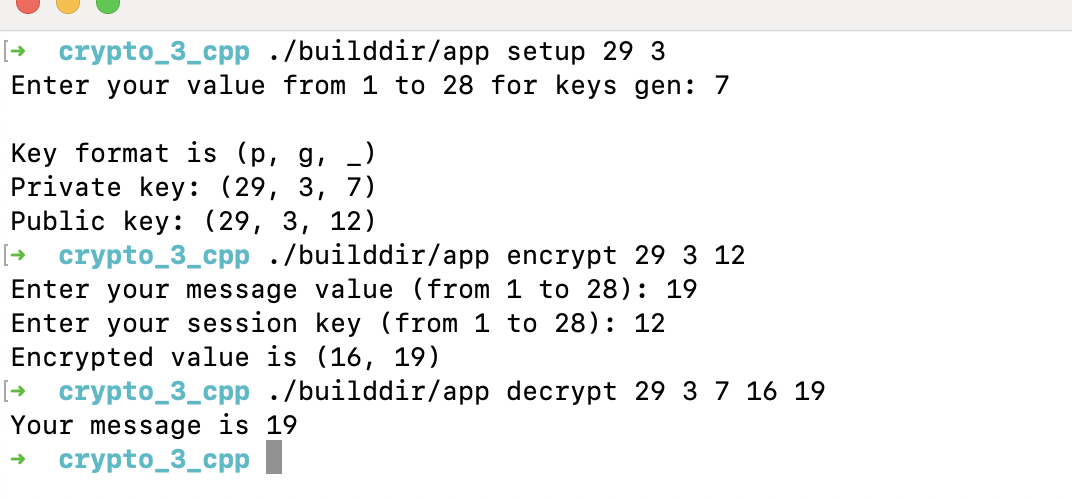
\includegraphics[width=\textwidth]{15_1}
  \end{figure}

  \subsubsection{Пример на больших числах}

  \begin{figure}[H]
    \centering
    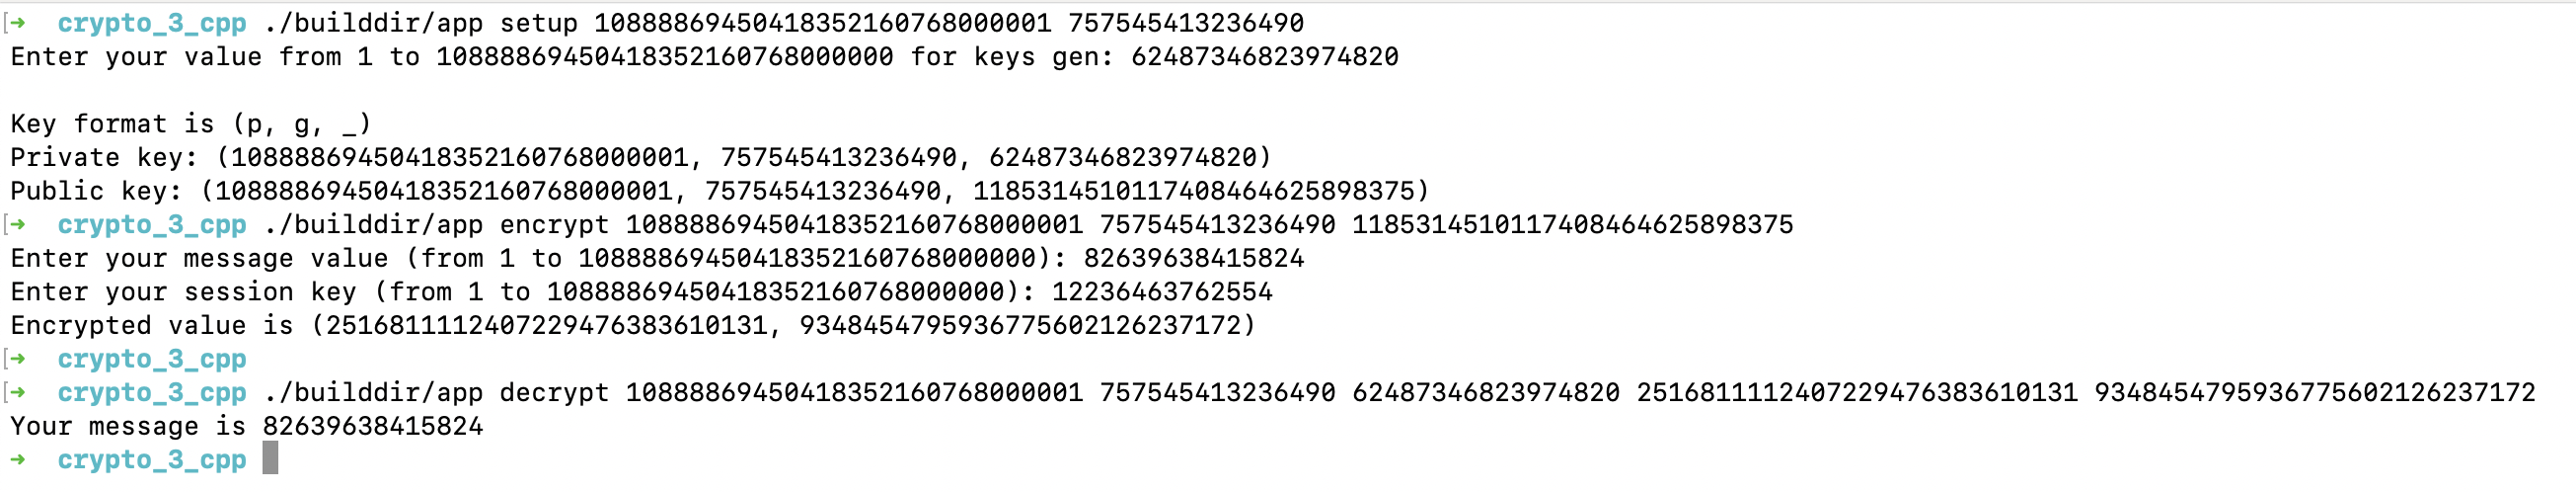
\includegraphics[width=\textwidth]{15_2}
  \end{figure}

  \section{Криптоанализ}

  \subsection{Метод грубой силы}

  Как любая криптографическая система, система Эль-Гамаля может быть взломана полным перебором.
  В связи с тем, что в качестве параметров домена могут быть выбраны очень большие числа, такая
  атака будет слишком долгой.

  Перебирать в данном случае можно как значения для закрытого ключа, так и сессионное значение.

  \subsection{Атака на основе подобранного шифр-текста}

  Если происходит зашифрование относительного маленького значения $m$, то вероятно получить ситуацию,
  при которой:
  \begin{equation}
    E(m) = (C_1, C_2)
  \end{equation}
  \begin{equation}
    E(2m) = (C_1, 2C_2)
  \end{equation}
  где $E(m)$ - операция зашифрования сообщения $m$.

  При помощи данной атаки не получится сделать какие-либо выводы о закрытом ключе
  или использованном при зашифровании сессионном значении, однако благодаря ей можно
  подменить реальное значение на фальсифицирован-ное:

  \begin{figure}[H]
    \centering
    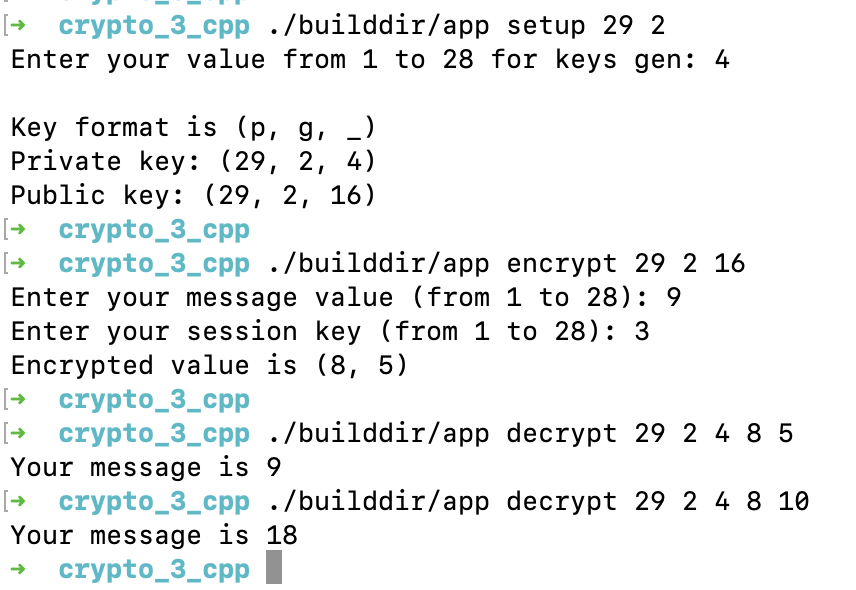
\includegraphics[width=0.7\textwidth]{15_3}
  \end{figure}

  В данном примере демонстрируется, как можно, подав на расшифрование
  пару $(C_1, 2C_2)$ вместо $(C_1, C_2)$ можно получить сообщение $2m$ вместо $m$.

  \subsection{Алгоритмы ускоренной факторизации}

  Стойкость данной системы основывается на сложности факторизации це-лых чисел, то есть
  на сложности решения уравнение вида:
  \begin{equation}
    a^x = b \mod{p}
  \end{equation}
  где известны все величины, кроме $x$.

  В данной системе факторизация применима к вычислению сессионного значения из выражения вида:
  \begin{equation}
    C_1 = g^k\mod{p}
  \end{equation}.

  Как и в условии, величины $C_1$, $g$ и $p$ известны, если найти значение $k$,
  то исходное сообщение можно найти по формуле:
  \begin{equation}
    C_2 \cdot h^{-k} = m\cdot h^k \cdot h^{-k} = m
  \end{equation}

  Существуют алгоритмы, позволяющие выполнить факторизацию за вре-мя, ассимптотически описываемое как $O(\sqrt{p}\log{p})$:

  С его помощью можно успешно вычислять зашифрованное сообщение в системах с относительно небольшим значением $p$, зная только шифр-текст и открытый ключ.
  
  \newpage
  Ниже приведена программная реализация дискретного логарифмирования с указанной сложностью:
  \begin{minted}{c++}
auto DiscreteLog(bigint a, bigint b, bigint p) -> bigint {
    bigint h = big_sqrt(p) + bigint(1);
    bigint c = PowMod(a, h, p);

    std::unordered_map<std::string, bigint> uToi;

    bigint lastCDegree = c;
    for (bigint i(1); i <= h; i++) {
        uToi[lastCDegree.asStr()] = i;
        lastCDegree = (lastCDegree * c) % p;
    }

    bigint lastV = b;
    for (bigint i(0); i <= h; i++) {
        if (uToi.contains(lastV.asStr())) {
            bigint v = i, u = uToi[lastV.asStr()];
            return h * u - v;
        }
        lastV = (lastV * a) % p;
    }

    throw std::invalid_argument("sorry, cant");
}
  \end{minted}

  \begin{figure}[H]
    \centering
    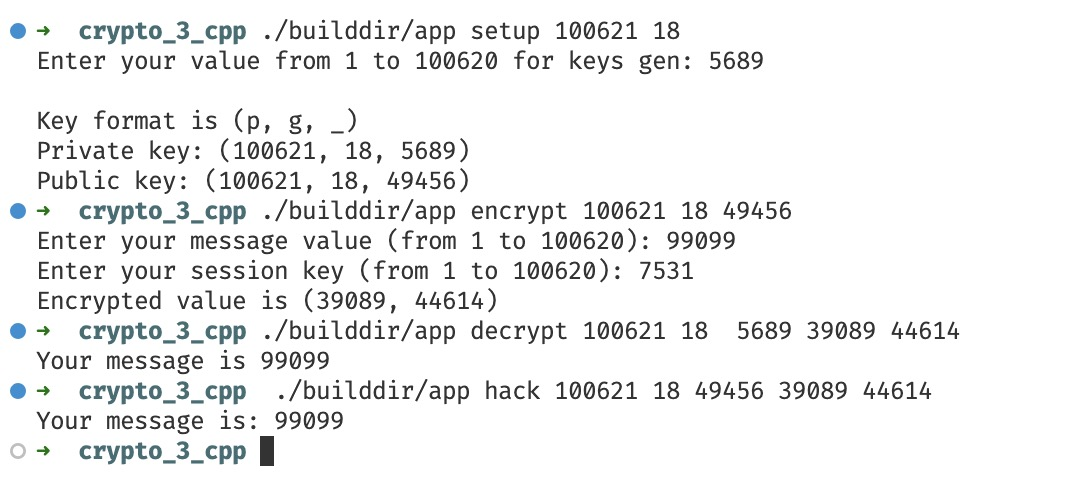
\includegraphics[width=\textwidth]{15_4}
    \caption{Расшифрование без закрытого ключа, вариант 1}
  \end{figure}

  \begin{figure}[H]
    \centering
    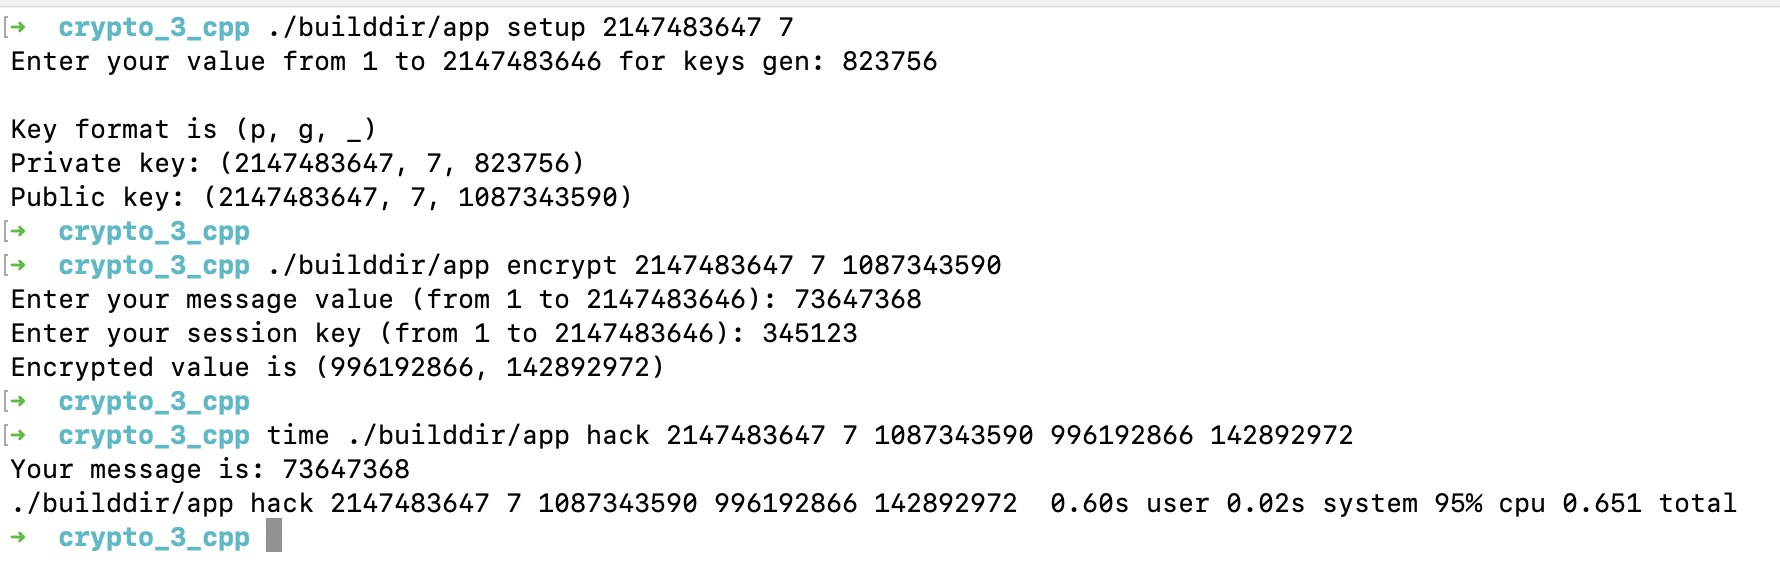
\includegraphics[width=\textwidth]{15_5}
    \caption{Расшифрование без закрытого ключа, вариант 2}
  \end{figure}

  Видим, что при решении задачи факторизации, расшифрование без зна-ния закрытого ключа не составляет проблемы.
  Для $p = 67280421310721$ время взлома составило приблизительно 3 минуты:
  \begin{figure}[H]
    \centering
    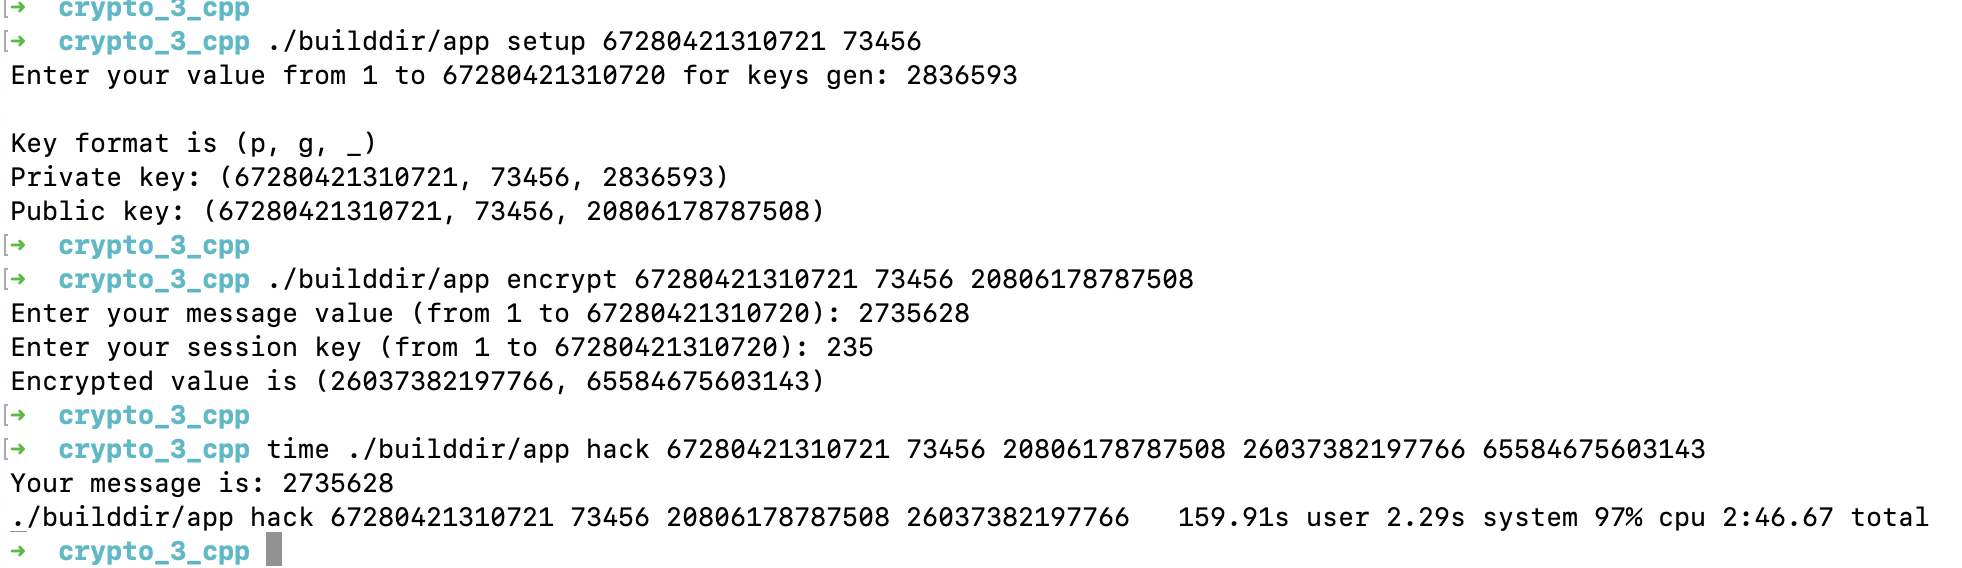
\includegraphics[width=\textwidth]{15_6}
    \caption{Расшифрование без закрытого ключа, вариант 3}
  \end{figure}

  \newpage
  \section{Вывод}

  В ходе данной работы были разобраны принципы действия криптосисте-мы Эль-Гамаля,
  произведена ее программная реализация и выполнен крипто-анализ.

\end{document}
